\chapter{Sparse coding}
\label{chap:sparse_coding}
%Back to our initial problem of\ref{sec:dicts} $x = D\alpha$

A sparse code is a sparse vector of coefficients that is used 
to linear combine a small selection of atoms from a dictionary.
Consider $X \in \mathbb{R}^{m\times n}$  as a matrix with $n$ columns each
column $x_{i}$ representing a signal described by a single vector of
signal length $m$. The dictionary $D\in\mathbb{R}^{m \times p}$ is another
matrix with $p$ columns where each column represents an atom signal with the
same dimension as a single signal $x_{i}$ from $X$. The number of 
atoms $p$ in the dictionary is higher then the dimension $m$ of the signals
$p > m$ making the dictionary over-complete. The sparse vector $\alpha$ consists
of coefficients that can describe a linear combination of only a few
non-orthogonal atoms from $D$ that is close to the signal $X$. 

%Sparse coding is the 
\begin{align}
X = \underbrace{\begin{pmatrix} x_1 \\ x_2 \\ \vdots \\ x_n
\end{pmatrix}}_{signal}
\approx \underbrace{\begin{pmatrix} d_1  d_2 \cdots d_n
\end{pmatrix}}_{\textrm{dictionary atoms}}
\underbrace{\begin{pmatrix} \alpha_1 \\ 0 \\ \vdots \\ \alpha_n
\end{pmatrix}}_{\textrm{sparse vector}}
\end{align}

%Or in other words ...
%\begin{equation}
%x = D\alpha+\epsilon \notag\\
%\end{equation}

The solution to this problem is a least-squares solve of an under-determined
linear system.
\begin{equation}
\min_{\alpha\in\mathbb{R}^{p}} \underbrace{\lVert x - D\alpha
\rVert^{2}_{2}}_{error} \label{eq:problem}
\end{equation}
The problem is not well-posed because there is more than one
solution to it. Such a problem is called a ill-posed problem.
But instead off all solutions we want to find the sparsest
solution making the problem well-posed. To archive this it is necessary to keep
the coefficient vector $\alpha$ sparse. Which means that only a few coefficients
of $\alpha$ are non-zero. 
\begin{figure}[h]
\centering
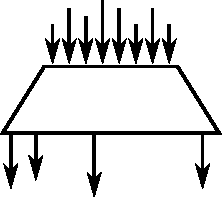
\includegraphics[width = 0.20\textwidth]{images/sparse.pdf}
\caption{over-complete and sparse}
\label{fig:sparse}
\end{figure}

\begin{figure}[h]
\centering
%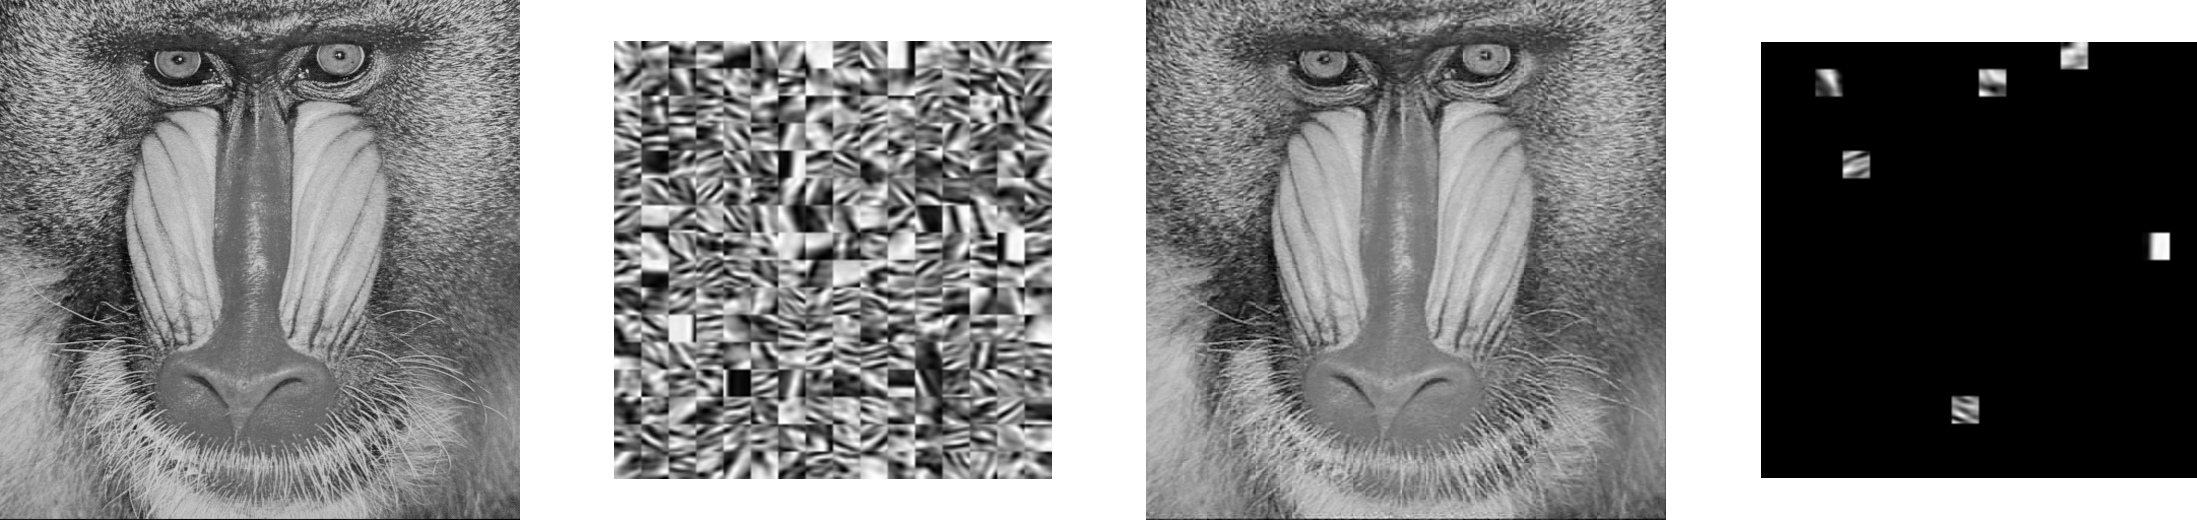
\includegraphics[width = 1.0\textwidth]{images/sparse_selection.pdf}
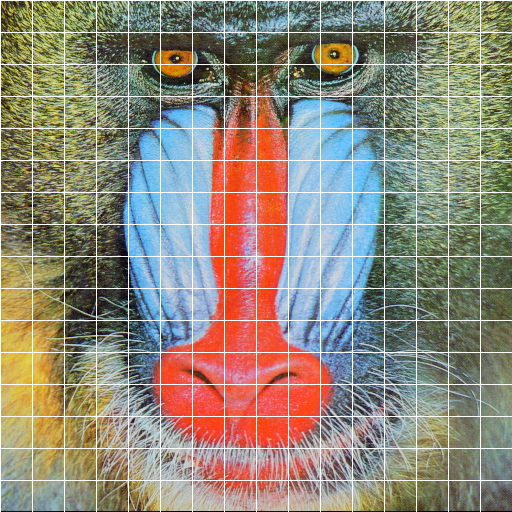
\includegraphics[scale = 0.25]{images/segmentation.png}
\caption{}
\label{fig:sparse}
\end{figure}
The idea of sparse coding image signals has its origin in neural science. 
Research in this field found that the cells in the visual cortex, also known as
\emph{V1}, have properties similar to those localized filtering of wavelets
functions. Several approaches were made to create system that resemble this
phenomena but did not lead to the desired structures. In 1996 Olshausen and
Field\cite{Olshausen1996} noticed that when adding a sparsity constraint to
these learning algorithms they can regenerate those characteristic elements.
Following this discovery constraints were added to the least-squares problem.


\section{Regularization}
A regularization adds additional information to a problem in order to solve an
ill-posed problem or to prevent over-fitting.\footnote{\url{
http://en.wikipedia.org/wiki/Regularization_(mathematics)}}
To find the sparsest solution the sparse coding approach adds such
regularization to the the least-squares problem\ref{eq:problem}. 
%.. over-fitting .. Such a constraint is the regularization.
\begin{equation}
\min_{\alpha\in\mathbb{R}^{p}} \lVert x - D\alpha \rVert^{2}_{2} +
\underbrace{\psi(\alpha)}_{regularization}
\end{equation}
The regularization acts a constraint to the structure of $\alpha$. It should be
choosen in a way which keeps the number of non-zero coefficient of $\alpha$ low.
This sparsity constraint can be achieved with the help of the $\ell_0$-norm.
The $\ell_0$-norm is a pseudo-norm that virtually counts the number of non-zero
elements in the vector in the form of:
\begin{equation}
\lVert\alpha\rVert_{0} = \#\{i:\alpha_i \neq 
0,i=1,...,p,\alpha\in\mathbb{R}^p\} 
\end{equation}
There is one significant problem in using $\ell_0$-norm. This particular
regularization makes the initial problem \ref{eq:problem} NP-hard. To get the
ideal solution it is necessary to test every combination of atoms. But this
does not imply that there is no way to efficiently find a solution that is good
enough to keep $\alpha$ sparse. There exist several greedy algorithms that can
solve the problem in a not perfect but good enough way. 

Another regularization that can keep $\alpha$ sparse is the use of the $\ell_1$
or $\ell_2$-norm as a convex relaxation of the $\ell_0$-norm. Even though that
the $\ell_1$-norm is not the same as the $\ell_0$ it can be demonstrated that
the $\ell_1$-norm is equivalent to the $\ell_0$-norm in the effect of inducing
sparsity.
\Todo{image/description of different regularizations}
\begin{figure}[h]
\centering
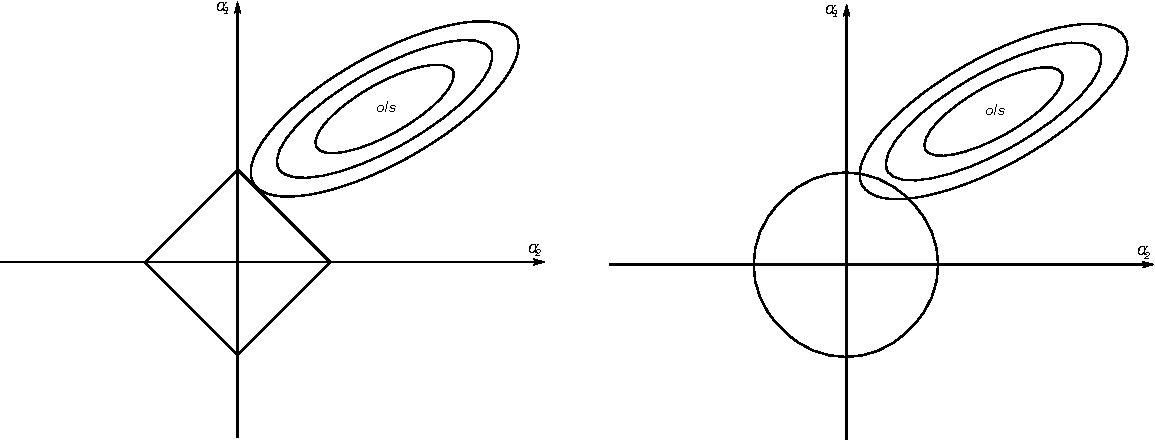
\includegraphics[width = 0.44\textwidth]{images/regularization.pdf}
\caption{sparse solution is approaching ordinary-least-squares solution}
\label{fig:sparse}
\end{figure}

In the last 15 years several sparse coding algorithms have been proposed. Some
that solve the initial $\ell_0$ regularized problem greedily, like
the (orthogonal)-matching-pursuit, and others which modified the problem to
become convex. The algorithms solve the convex problem  primary derived from the
numerical domain in the form of large linear system solvers with few
optimization constraints. The most common of them are the Basis-pursuit,
LARS-Lasso, Ridge regression and FOCUSS. The next two sections give a more in
depth look on those algorithms. 

%$\ell_2$ Method Of Frames


%copy
% Following Tao et al., where it was shown that the L1 norm is equivalent to the
%L0 norm, 
%leads one to solve an easier problem. Finding the candidate with the smallest
%L1 norm can be expressed relatively
%easily as a linear program, for which efficient solution methods already exist.
%These solution methods have been refined over the past few years yielding
% enormous gain
%\begin{figure}
%\centering
%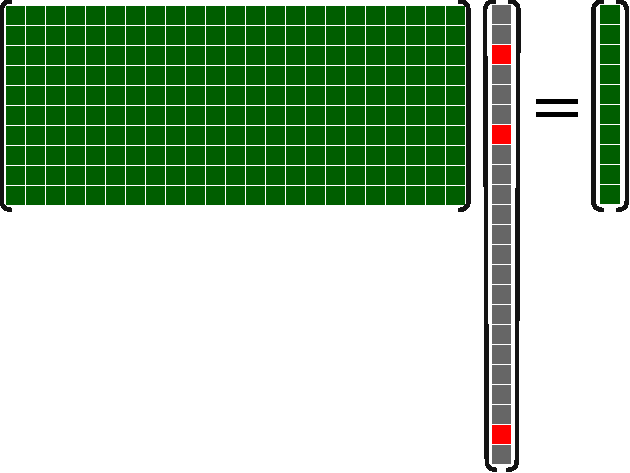
\includegraphics[width = 0.66\textwidth]{images/Da_x.pdf} % Or .pdf
%\caption{Sparse Coding}
%\label{fig:da_x}
%\end{figure}

\section{$\ell_0$ regularization with greedy algorithms}
%present a selection of the most common algorithms to solve the initial problem
%under a $\ell_0$ regularization.
We now give a more in depth look at two very popular algorithms. 
The matching-pursuit and its successor the orthogonal-matching-pursuit.
Both use a greedy strategy to calculate the coefficient vector $\alpha$ to find
a solution to the following NP-hard problem.
\begin{equation}
\min_{\alpha\in\mathbb{R}^{p}}   \lVert \alpha \rVert_{0}   \textrm{ s.t. }
\lVert x - D\alpha \rVert^{2}_{2} \leq \epsilon
\end{equation}
respectively
\begin{equation}
\min_{\alpha\in\mathbb{R}^{p}}  \lVert x - D\alpha \rVert^{2}_{2} \textrm{ s.t.
} \lVert \alpha \rVert_{0} \leq L
\end{equation}
\cite{Mallat1993}

\subsection{Matching-Pursuit}
\label{sec:mp}
The matching-pursuit was first presented in 1993 by Mallat and
Zhang\cite{Mallat1993} on audio samples and later adapted to images by Mallat
and Bergeaud in\cite{Mallat1995}.
The \prettyref{alg:mp} starts with the coefficient vector $\alpha$ set to
zero. Then finds the atom in the dictionary with the best reduction of the
error. This is done by selecting the coefficient that has the maximum
correlation with the current residual. This step is repeated $L$ times
or until the error $\lVert x - D\alpha \rVert^{2}_{2}$ for the current $\alpha$
reaches $\lVert x - D\alpha \rVert^{2}_{2} \leq \epsilon$ respectively the
residual fulfills $\lVert r \rVert_2 \leq \epsilon$.
\begin{algorithm}[H]
\caption{Matching Pursuit}
\label{alg:mp}
\begin{algorithmic}[1]
\REQUIRE $x \in \mathbb{R}^m, D \in \mathbb{R}^{m\times p}, L \in \mathbb{N},
\epsilon \in \mathbb{R}$
\STATE $\alpha_0 \gets 0$ (start with zero vector)
\STATE $r_0 \gets x-D\alpha_0 = x$ (residual) 
\WHILE {$\lVert \alpha \rVert_{0} \leq L$ $\lVert r \rVert_2 \leq \epsilon$}
\STATE Select atom with maximum correlation with residual: 
\begin{equation*}
i \gets \argmax_{i=1,...,p} \lvert \left<d_i,r\right> \rvert
\end{equation*}
\STATE update coefficients: 
\begin{align}
a[i]  \gets a[i] + \left<d_i,r\right> \label{eq:mp_update}
\end{align}
\STATE update residual:
\begin{equation*}
 r \gets r - \left<d_i,r\right>d_i
\end{equation*}
\ENDWHILE
\RETURN $\alpha$
\end{algorithmic}
\end{algorithm}

\subsection{Orthogonal-Matching-Pursuit}
\label{sec:omp}
The Orthogonal-Matching-Pursuit, an improved version of
the Matching-Pursuit (\ref{sec:mp}), was first presented by Pati et al.
in 1993\cite{Pati1993}. Rather than just updating the coefficient of $\alpha$
,that is currently selected (\ref{eq:mp_update}), the algorithm re-evaluates
all coefficient in the current set $A$ of active atoms 
$\alpha_A$ by solving a full least-squares solution in every iteration
(\ref{eq:omp_update}). This improves the quality of the
solution\cite{Pati1993}. The Orthogonal-Matching-Pursuit gets its name from
the fact that the residual $r$ is orthogonal to the previously selected atoms
in dictionary $D$. This orthogonality property leads to the effect that every
coefficient is only selected once. A description in pseudo-code is shown in
algorithm \ref{alg:omp}.
\begin{algorithm}[H]
\caption{Orthogonal Matching Pursuit}
\label{alg:omp}
\begin{algorithmic}[1]
\REQUIRE $x \in \mathbb{R}^m, D \in \mathbb{R}^{m\times p}, L \in \mathbb{N},
\epsilon \in \mathbb{R}$
\STATE $\alpha \gets 0, r \gets x $ (residual) $, A \gets \emptyset$
\FOR {$j = 0$ to $L$}
\STATE Select inactive variable with maximum correlation with residual: 
\begin{equation*}
i \gets \argmax_{i \in A^C} \lvert \left<d_i,r\right> \rvert
\end{equation*}
\STATE update active set:
\begin{equation*}
 A \gets A \cup \{i\} 
\end{equation*}
\STATE update coefficients: 
\begin{align}
a_A \gets \left( D_A^T D_A \right)^{-1} D_A^T x  \label{eq:omp_update}
\end{align}\label{alg:OMP_DTD}
\STATE update residual:
\begin{equation*}
 r \gets x-D_Aa_A
\end{equation*}
\ENDFOR
\RETURN $\alpha$
\end{algorithmic}
\end{algorithm}
%Section \ref{sec:batch-omp} provides a depper look into the Batch-OMP.

All these greedy approaches tend to find suitable solutions but
because of the non-convex problem they can get stuck in local minima. As shown
before an $\ell_1$ regularization version of \ref{eq:problem} also keeps the
coefficient vector $\alpha$ sparse but eliminates the problem of a local minima.
The next section presents algorithms which solve  a $\ell_1$ regularization
version of \ref{eq:problem}.


\section { $\ell_1$asso regularization}
The $\ell_1$ regularization of our initial problem is also known as the
\emph{Lasso}. The name stands for \emph{least absolute shrinkage and
selection operator} and is a regularized version of a least squares
solution. The sparsity is achieved by adding a constraint that induces
the $L_1$-norm of the solution to be small. It was first presented by Tibshirani
in 1996\cite{Tibshirani1996}. Under this constraint our initial problem becomes:
\begin{equation}
\min_{\alpha\in\mathbb{R}^{p}} \lVert x - D\alpha \rVert^{2}_{2} \textrm{
s.t. } \lVert \alpha \rVert_{1} \leq L \label{eq:l1}
\end{equation}
The algorithms dealing with this problem often require to formulate the
constrained function into a single expression. The lagrange multiplier is a
method to construct such an expression from a function and the constraint. With
the  lagrange multiplier applied the regularized problem \ref{eq:l1} becomes:
\begin{equation}
\min_{\alpha\in\mathbb{R}^{p}}  \frac{1}{2} \lVert x - D\alpha \rVert^{2}_{2} +
\lambda \lVert \alpha \rVert_{1}\label{eq:l1lagrange}
\end{equation}
Where the coefficient $\lambda$ controls the sparsity equivalent to $L$.
In the last two decades several algorithms were proposed to compute the
Lasso. The basis pursuit by Chen et al.\cite{Chen1995}, the FOCUSS\cite{FOCUSS}
the LARS by Efron et al.\cite{Efron2004} among others.


\subsection {LARS-Lasso}
\label{sec:lars}
% \Todo{split into LAR and LARS-lasso, better illustrate than use complex
%formulas}
The LARS-Lasso was first presented in 2004 by Efron et al.\cite{Efron2004}.
It is a algorithm to solve the Lasso with the help of a regression
algorithm known as \emph{least-angle regression}. Regression tries to find the
correlation between a depended variable, here \prettyref{eq:l1lagrange}, and a
set of independent variables, our coefficients of $\alpha$.

\paragraph{Least-angle regression}
The main idea of the least angle regression is to start with all coefficient
zero $\alpha = 0$. Then find the variable $x_i$ with the maximum correlation
with the residual $r$ and move linear into the direction of the ordinary least
squares solution until a new variable has a higher correlation with the
residual.  
%The complete regularization path based on\cite{Efron2004}
\begin{align}
\min_{\alpha\in\mathbb{R}^{p}}  \frac{1}{2} \lVert x - D\alpha \rVert^{2}_{2} +
\lambda \lVert \alpha \rVert_{1}
\end{align}

\paragraph{Lasso modification}
The LAR algorithm can be easily modified to solve the Lasso. 
The modification consists of removing variables from the active set
when their coefficient become zero. A pseudocode implementation can be found in
\prettyref{alg:lars}.
\begin{algorithm}
\caption{LARS-Lasso}
\label{alg:lars}
\begin{algorithmic}[1]
\REQUIRE $x \in \mathbb{R}^m, D =[d_1,...,d_p] \in \mathbb{R}^{m\times p}, L \in
\mathbb{N}, \epsilon \in \mathbb{R}$
% xD normalized and centered
\STATE $\alpha \gets 0, \mu_{0} \gets 0, A \gets \emptyset$
\FOR {$j = 0$ to $L$}
\STATE calculate correlations with residual: $c \gets D^t\left( x-\mu_j \right)
$
\STATE Select atom with maximum correlation: 
\begin{equation*}
i \gets \argmax_{i \in A^C} \lvert c_i  \rvert % \left<d_i,x-\mu_{j}\right>
\end{equation*}
\STATE maximum correlation: $c_{max} \gets c_i $ %\left<d_a,r\right> $
\STATE update active set: $A \gets A \cup \left\{i\right\} $
\STATE calculate movement into OLS direction:
\STATE signs of the correlations: $s_A \gets  sign\left(c_A\right)$
\STATE $\tilde{D_A} \gets D_A\left(\ldots s_id_i \ldots\right)_{i\in A}$
\STATE $G_A \gets \tilde{D_A}^T\tilde{D_A}$
\STATE calculate angle: $A_A \gets \sqrt{ 1_A^{-1} G_A^{-1} 1_A
}$
\STATE apply weights: $w_A \gets A_AG_A^{-1}1_A$
\STATE equiangular direction: $u_A \gets D_Aw_A$
\STATE correlation between direction and variables: $a \gets D_tu_A$
\STATE minimal movement:
\begin{equation*}
\gamma \gets \min_{i\in A^C}^{+} \left\lbrace \frac{c_{max}-c_i }{A_A-a_i },
\frac{c_{max}+c_i }{A_A+a_i } \right\rbrace
\gamma \gets \min_{i\in A^C}^{+} \left\lbrace \frac{c_{max}-\left< x,d_i
\right> }{1-\left< d_a,d_i \right> }, \frac{c_{max}+\left< x,d_i \right>
}{1+\left< d_a,d_i \right> } \right\rbrace
\end{equation*}
\STATE drop coefficient from active that change sign: 
\STATE $ \tilde{\gamma} \gets -\alpha/s_A^Tw_A  $
\STATE $ i \gets \min_{i\in A}^{+} \left( \tilde{\gamma}_i \right) $
%\STATE $ i \gets \alpha_{i} = 0, i \in A $
\IF {$\tilde{\gamma}_i>0$ and $\tilde{\gamma}_i<\gamma$}
\STATE remove from active set: $ A \gets A \backslash \{i\} $
\STATE update movement: $ \gamma \gets \tilde{\gamma} $  
\ENDIF
%\STATE $ \mu_{j+1} \gets \mu_{j} - \gamma x_i $
\STATE $ \mu_{j+1} \gets \mu_{j} - \gamma u_a $
\STATE $ \alpha \gets \alpha - \gamma s_A^Tw_A $
\ENDFOR
\end{algorithmic}
\end{algorithm}


\paragraph{Limitations}
We have to admit that the LARS-Lasso algorithm some limitations.
\begin{description}
 \item[Dimension] When the dimension $p$ of the signal $X$ is much higher than
the the dimension $m$ of the dictionary $D$ the algorithm can only select $m$
columns.
  \item[Correlation] When the columns of the dictionary are highly correlated
the algorithm selects only one column.
\end{description}
The first limitation is not relevant for our experiments as our dictionaries
are over-complete, with respect to the dimension $m$ of signal $X$, and thus
satisfy $p\leq n$. 

\section{Application and Related Work}
In the most applications and papers related to sparse coding,the coding
step and the dictionary learning step are often close tied together. This
section concentrates on work where the sparse coding step is dominating. Section
\ref{sec:related_dictionarie} show related work where the learning of
dictionaries is the dominating part of the work.

%\begin{description}
\paragraph{Noise reduction}
Elad and Aharon\cite{Elad2006}
Remove noise from a signal. 
Using the fact that sparse coding is an approximation of signal that loses ...
noise? ... in its encoding process. 
\begin{align*}
y = x + w
\end{align*}

\paragraph{In-painting}
fill missing parts by removing rows from the dictionary
Train with the original image
\begin{align*}
x \approx D\alpha\\
x_s \approx D_s\alpha\\
Wx \approx WD\alpha\text{select subset}\\
\end{align*}
\cite{mairal08sparse}


%Task driven dictionaries

\paragraph{Inverse half-toning} Half-toning, as used in printing ,is a process
where binary raster simulates continuous tone images. Small dots of different
size and shape create the optical illusion of continuous tones. In 2010 research
by Mairal et al.\cite{Mairal2010b} presented 


\paragraph{Super resolution} \cite{Wright2008,Yang2010, Yang2010}  
Or the ongoing work by Couzinie-Devy et al., 2010 called digital zooming.

\paragraph{Background subtraction}\cite{}

\paragraph{Edge detection}\cite{Mairal2008c}

\paragraph{Sense sparse signals}\cite{Duarte2009}
%\item[noise reduction]
%\item[in-painting]
%\item[classification] \Todo{usage:classification}
%\end{description}







